\documentclass{article}

\usepackage[utf8]{inputenc}
\usepackage[T1]{fontenc}
\usepackage{datetime}
\usepackage{graphicx}
\usepackage{float}
\usepackage{subcaption}

\usepackage{minted}
\usepackage[os=win]{menukeys}
\usepackage{tikz}

\usepackage[english]{babel}
\usepackage{geometry}

\usepackage{adjustbox}
\usepackage{multirow}
\usepackage{hyperref}
\usepackage{titlesec}

\geometry{
	a4paper,
	left=25mm,
	right=25mm,
	top=25mm,
	bottom=25mm,
}

\hypersetup{
	colorlinks=true,
	linkcolor=blue,
	urlcolor=blue,
}

\setcounter{secnumdepth}{4}
\renewcommand{\theparagraph}{\thesubsubsection.\alph{paragraph}}

\addto\captionsenglish{\renewcommand{\contentsname}{Daftar Isi}}
\addto\captionsenglish{\renewcommand{\tablename}{Tabel}}
\addto\captionsenglish{\renewcommand{\figurename}{Gambar}}

\def\mydate{\leavevmode\hbox{\the\year-\twodigits\month-\twodigits\day}}
\def\twodigits#1{\ifnum#1<10 0\fi\the#1}

% this custom commands below will not work if not run on GNU/Linux
\newcommand{\ShowOsVersion}{
	\immediate\write18{\unexpanded{foo=`uname -srom | tr '_' '-'` && echo -n "${foo}" > tmp.txt}}
	\unskip\unskip\input{tmp.txt}\unskip
	\immediate\write18{rm tmp.txt}
}
\newcommand{\ShowTexVersion}{
	\immediate\write18{\unexpanded{foo=`pdflatex -version | head -n1 | cut -d' ' -f1,2` && echo -n "${foo}" > tmp.txt}}
	\unskip\unskip\input{tmp.txt}\unskip
	\immediate\write18{rm tmp.txt}
}

\begin{document}
\begin{titlepage}
		\centering

		{
			\LARGE
			\bf
			Laporan Kegiatan Pengujian Audiometri Portable
		}

		\bigskip

		{
			\large
			\bf
			Tim Penelitian Audiometer Portable Elbicare
		}

		\vfill

		\begin{figure}[H]
			\centering
			
\includegraphics[width=250pt,angle=0]{images/elbicare-logo}
		\end{figure}

		\vfill

        \bigskip

        {
            \bf
            Achmadi, S.T., M.T. dan M. Ammar Asyraf, S.T.
        }
	\end{titlepage}

	\newpage

	\textbf{Tentang Dokumen}\\

	\noindent Dokumen ini ditulis menggunakan {\textbf{\ShowTexVersion}} pada sistem operasi {\textbf{\ShowOsVersion}} yang diupdate terakhir pada tanggal {\mydate} di jam \currenttime.\\

	\noindent Kode sumber dokumen ini dapat ditemukan di laman repositori proyek
	\url{https://github.com/VibrasticLab/pikoakustik2/tree/master/prototrial/dokumen/berita_acara/itb_july2023/test_calib}.

	\newpage

	\tableofcontents

	\newpage
	
	{\large \bf Informasi Kegiatan Pengujian}
	
	\begin{table}[H]
		\centering
		\begin{tabular}{p{0.35\linewidth} p{0.01\linewidth} p{0.4\linewidth}}
			Identitas Penguji & : & 1. Achmadi, S.T., M.T. \newline 2. Muhammad Ammar Asyraf, S.T.\\ \hline
			Nama Alat & : & Audiometer Portabel\\ \hline
			Merk & : & eLBicare\\ \hline
			Model & : & v3.0\\ \hline
			Nomor Seri & : & - \\ \hline
			Tempat (Ruangan) & : & Laboratorium Akustik Adhiwijogo, Teknik Fisika ITB Bandung \\ \hline
			Tanggal Pelaksanaan & : & 10 - 12 Juli 2023\\ \hline
			Identitas Fasyankes / Pelanggan & : & Poli Audiologi RSUD Dr. Soetomo Surabaya\\ \hline
		\end{tabular}
	\end{table}
	
	
	\section{Pendahuluan}

	Dokumen ini merupakan laporan hasil kegiatan pengujian perangkat audiometer berdasarkan Metode Kerja Balai Pengamanan Fasilitas Kesehatan (MK-BPFK) No. 007-18 tentang Metode Kerja Pengujian Audiometer.  

	\subsection{Tujuan Kegiatan}

	Tujuan utama kegiatan ini adalah melakukan pengujian dan/atau kalibrasi secara langsung (direct calibration) pada
	{\bf eLBicare Portable Audiometer v3.0}, dengan cara melakukan pemeriksaan fisik, pengujian fungsi, pengujian keselamatan listrik dan pengukuran
	kinerja (kalibrasi).
	
	\subsection{Ruang Lingkup Pengujian}
	
	Pelaksanan pengujian audiometer yang dilakukan mengalami penyesuaian dari MK BPFK yang digunakan, dengan mempertimbangkan kondisi aktual perangkat audiometer yang diujikan dan ketersediaan alat ukur yang tersedia. Metode pengukuran yang kemudian dilaksanakan memiliki lingkup pengujian sebagai berikut:
	\begin{enumerate}
		\item Perangkat Audiometer yang diuji merupakan perangkat portable bertenaga baterai (battery power)
		
		\item Perangkat Audiometer Portabel yang diuji hanya memiliki opsi pengujian air conduction
		
		\item  Algoritma perangkat audiometer portable yang digunakan adalah metode Three-Forced Choice (3AFC)
	\end{enumerate}

	\noindent Adapun ruang lingkup pengujian yang dilakukan meliputi aspek-aspek berikut.
	\begin{enumerate}
		\item Pemeriksaan fisik
		
		\item Pengujian fungsi
		
		\item Pengujian keselamatan listrik
		
		\item Pengujian kinerja, meliputi:
		\begin{enumerate}
			\item Hearing level Air Conduction
			
			\item Akurasi Frekuensi
			
			\item Total Harmonic Distortion Air Conduction
		\end{enumerate}
		
	\end{enumerate}

	\subsection{Waktu dan Tempat}

	Kegiatan ini dilakukan di Ruang Dengung dan Ruang Kedap Laboratorium Akustik Adhiwijogo di Institut Teknologi Bandung pada tanggal 10-12 Juli 2023.

	\subsection{Alat dan Perlengkapan}

	Alat yang digunakan meliputi:
	
	\begin{enumerate}
		\item Perangkat eLBicare Audiometer Portabel beserta headphone JBL Tune 500. Berikut laman produk: \href{https://id.jbl.com/over-ear-headphones/JBL+TUNE500.html}{JBL Tune 500}
		
		\item Speaker merek Yamaha dengan Amplifier board portabel.

		\item Sound Level Meter Merek Rion yang telah terkalibrasi.

		\item Unit MiniDSP EARS sebagai Simulator Telinga. Ini adalah unit simulator telinga pertama.
		Berikut laman produk: \href{https://www.minidsp.com/products/acoustic-measurement/ears-headphone-jig}{MiniDSP EARS}

		\item Unit Microphone 3DIO dan AudioBox Presonus USB96. Ini adalah unit simulator telinga kedua.
		Berikut laman produk: \href{https://3diosound.com/products/free-space-pro-binaural-microphone}{3DIO}
		dan \href{https://www.frontendaudio.com/presonus-audiobox-usb-96-usb-audio-interface/}{AudioBox USB96}

		\item Perangkat Lunak Audacity dan RealTime Analyzer dari Yoshimasa.
		Berikut laman produk: \href{https://www.audacityteam.org/}{Audacity} dan \href{http://www.ymec.com/products/dssf3e/}{RTA}.
	\end{enumerate}

	\subsection{Kondisi Lingkungan}
	
	Kondisi lingkungan saat pelaksanaan kegiatan adalah sebagi berikut.
	
	\begin{table}[H]
		\begin{tabular}{p{0.3\linewidth} p{0.01\linewidth} p{0.4\linewidth}}
			Suhu Lingkungan & : & \ldots \\ 
			Kelembapan & : & \ldots \\ 
			Voltasi Instalasi Listrik Medis & : & N/A\\ 
		\end{tabular}
	\end{table}	

	\newpage
	\section{Prosedur Kegiatan}
	
	\subsection{Kegiatan Pra-Pengujian}
	
	\subsubsection{Persiapan dokumen}
	\begin{enumerate}
		\item Manual penggunaan alat dan perangkat lunak pengujian
		\item Metode kerja
		\item Lembar kerja
		\item Standar acuan pengujian
	\end{enumerate}

	\subsubsection{Persiapan alat yang akan di uji}
	\begin{enumerate}
		\item Perangkat eLBicare Audiometer Portabel disiapkan
		\item Kelengkapan aksesori (headphone JBL) diperiksa
	\end{enumerate}
	
	\subsubsection{Persiapan alat uji/kalibrasi}
	\begin{enumerate}
		\item Alat ukur keselamatan listrik disiapkan
		\item Alat Sound Level Meter (SLM) standar disiapkan
		\item Alat Sound Pressure Level (SPL) calibrator disiapkan
		\item Software interface SLM disiapkan
		\item Thermohygrometer disiapkan
	\end{enumerate}
	
	\subsubsection{Pendataan administrasi alat yang diuji}
	Poin yang perlu untuk didata adalah sebagi berikut.
	\begin{enumerate}
		\item Identitias penguji
		\item Nama alat
		\item Merek
		\item Model
		\item Nomor seri
		\item Ruangan
		\item Tanggal pelaksanaan
		\item Identitas Fasyankes/pelanggan
	\end{enumerate}
	
	\subsubsection{Pengukuran kondisi lingkungan}
	\begin{enumerate}
		\item Thermohygrometer dan electrical safety analyzer disiapkan 
		\item Suhu dan kelembapan ketika awal kegiatan dicatat
		\item Suhu dan kelembapan ketika akhir kegiatan dicatat
	\end{enumerate}
	
	\subsection{Pemeriksaaan Fisik dan Fungsi Alat yang Diuji}
	Pemeriksaan dan pengamatan fisik dan fungsi Audiometer dilakukan dengan mengikuti prosedur berikut.
	\begin{enumerate}
		\item Badan dan permukaan alat, periksa bagian luar unit, pastikan bersih, terpasang ketat satu dan lainnya dan tidak ada bekas tertimpa cairan ataupun gangguan lainnya.
		\item Kotak kontak alat, periksa apakah ada gangguan pada kotak kontak (AC-Power). Gerak-gerakkan kotak kontak untuk memastikan keamanannya. Goyang-goyangkan kotak kontak untuk memastikan tidak ada baut atau mur yang longgar.
		\item Kabel catu utama, Periksa kabel, apakah terlihat ada kerusakan atau bagian isolasi yang terkelupas.
		\item Sekering pengaman, Periksa sekering yang terdapat pada bagian luar rangkaian, apakah nilai tahanan dan tipenya sesuai dengan spesifikasi yang tertulis pada alat. Sekering pengaman harus berfungsi baik.
		\item Kabel elektroda, Periksa kabel dan fungsi masing-masing kedua ujungnya (kotak kontak) dan keregangannya secara menyeluruh. Kemudian periksa dengan hati-hati apakah terdapat luka ataupun sobek pada lapisan isolasinya, hal ini untuk menghindari adanya gangguan tegangan dan mencegah noise.
		\item Tombol, saklar dan kontrol, Sebelum mempergunakan/ mengubah-ubah tombol kontrol, periksa posisinya, jika terlihat tidak berada pada posisinya (periksa dengan menggunakan mode pemeriksaan standar). Bandingkan dengan posisi control. Ingat pengaturan tersebut dan jangan lupa untuk mengembalikan pada setting awal jika sudah selesai menggunakan.
		\item Tampilan dan indikator, Selama pengecekan fungsi, pastikan lampu indikator dan tampilan berfungsi seluruhnya, yakinkan bahwa bagian tampilan digital berfungsi
	\end{enumerate}
	
	\subsection{Pengujian Keselamatan Listrik}
	Prosedur mengacu pada MK Pengujian Keselamatan Listrik Nomor MK 001-18
	
	\subsection{Pengujian Kinerja}
	
	\subsubsection{Konfigurasi Pengujian}
	Pengujian dilakukan dengan menyusun eLBicare Audiometer Portabel dengan alat uji sesuai dengan gambar berikut.
	
	\begin{figure}[H]
		\centering
		\includegraphics[width=0.5\textwidth]{example-image}
		\caption{Konfigurasi pengujian}
	\end{figure}
	
	\subparagraph{Setup dan Pengaturan Perangkat}
	\begin{enumerate}
		\item Pasang Headphone pada unit EARS sebagaimana jika digunakan pada telinga manusia.
		Pastikan kiri dan kanan tidak terbalik.
		Pastikan Headphone menutup lubang telinga.
		
		\begin{figure}[H]
			\centering
			\begin{subfigure}[H]{0.4\textwidth}
				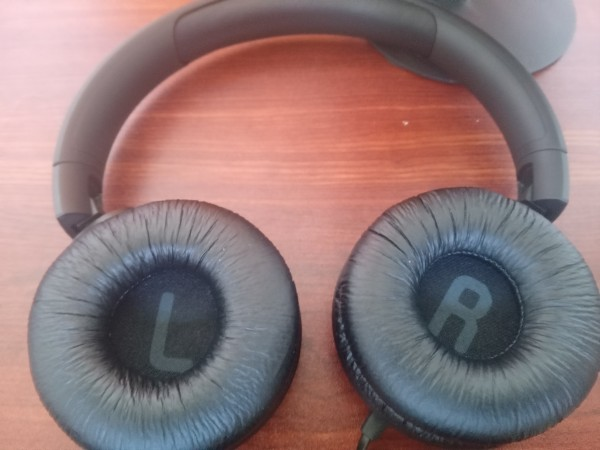
\includegraphics[width=\textwidth]{images/pasang/chjbl}
				\caption{Label Channel}
			\end{subfigure}
			\begin{subfigure}[H]{0.4\textwidth}
				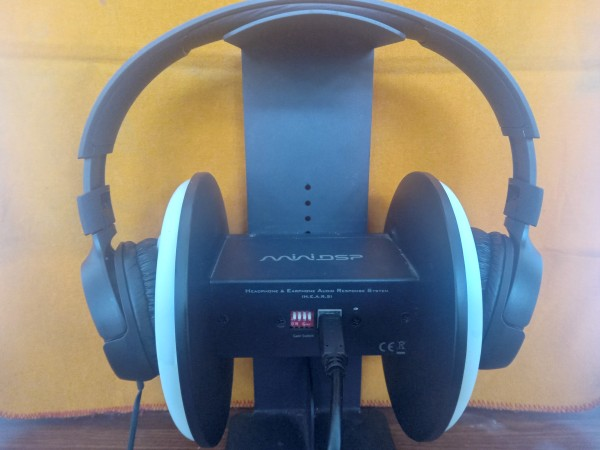
\includegraphics[width=\textwidth]{images/pasang/pasangjbl}
				\caption{Pasang Headphone}
			\end{subfigure}			
			\caption{Pemasangan Headphone pada EARS}
		\end{figure}
		
		\item Sambung Jack Audio Headphone ke Konsol
		\begin{figure}[H]
			\centering
			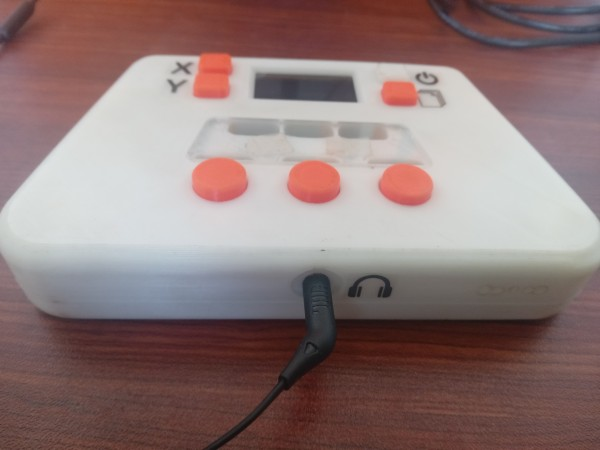
\includegraphics[width=200pt]{images/pasang/sambung_audio}
			\caption{Sambung Jack Audio}
		\end{figure}
		
		\item Nyalakan Unit. Tunggu hingga LED biru berkedip.
		\begin{figure}[H]
			\centering
			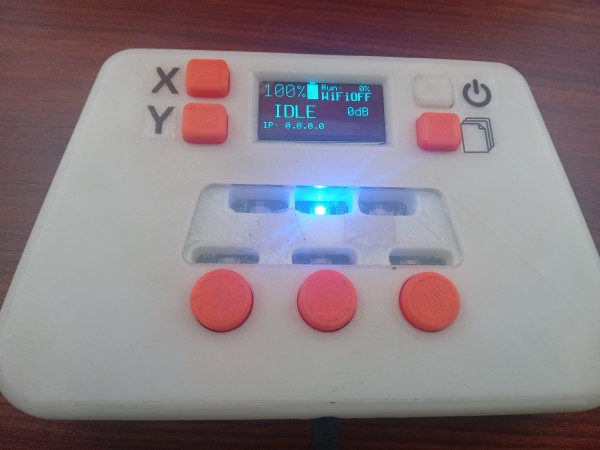
\includegraphics[width=200pt]{images/pasang/nyalakan_unit}
			\caption{Nyalakan Unit}
		\end{figure}
		\item Sambung Kabel USB ke Konsol
		\begin{figure}[H]
			\centering
			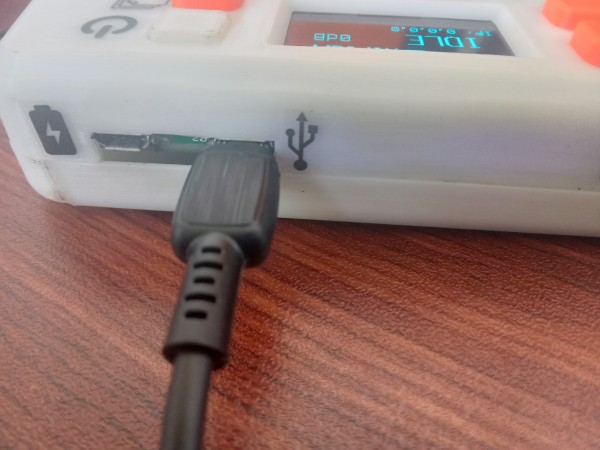
\includegraphics[width=200pt]{images/pasang/sambung_usb}
			\caption{Sambung Kabel USB}
		\end{figure}
	\end{enumerate}
	
	\subparagraph{Komunikasi Serial}
	
	\begin{enumerate}
		\item Berikut adalah perangkat lunak komunikasi serial ke Konsol yang perlu disiapkan untuk pengujian ini (panduan ini menggunakan Windows-7 32-bit sebagai contoh)
		
		\item Install driver ARM USB-CDC.\\
		Untuk dapat menghubungkan unit prototype dengan komputer,
		diperlukan driver ARM USB-CDC untuk komunikasi serial.
		
		\begin{itemize}
			\item File installer (sesuaikan dengan bit OS).
			Dapat didownload di \href{https://drive.google.com/drive/folders/19gXVrxR68SFHQUGGGgKb0Da03oV7Rh41?usp=share_link}{USB-CDC\_Driver}.
			\begin{figure}[H]
				\centering
				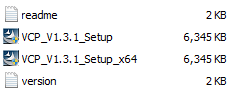
\includegraphics[width=200pt]{images/software/driver}
				\caption{Installer Driver}
			\end{figure}
			
			\item Instalasi driver (tanpa unit prototype terhubung) cukup mudah sebagaimana umumnya.
			\begin{figure}[H]
				\centering
				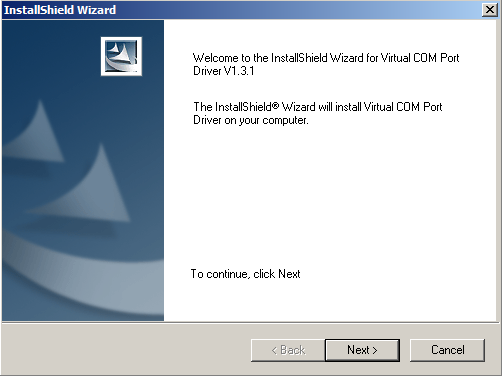
\includegraphics[width=200pt]{images/software/install_driver}
				\caption{Mulai instal driver}
			\end{figure}
		\end{itemize}
		
		\item Sambungkan unit prototype yang telah nyala dengan komputer via kabel USB.
		\begin{figure}[H]
			\centering
			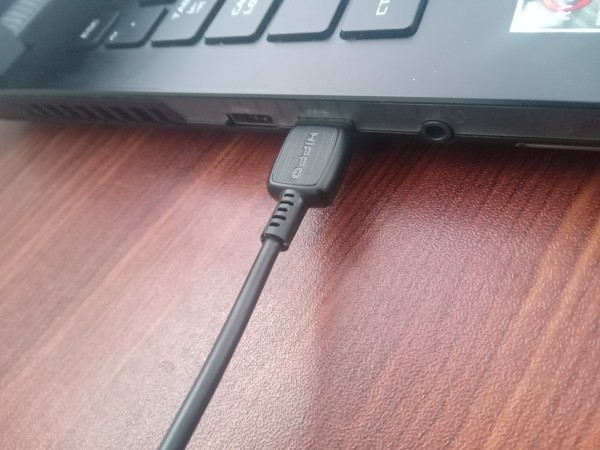
\includegraphics[width=200pt]{images/pasang/laptop_usb}
			\caption{Sambung Kabel USB ke Laptop}
		\end{figure}
		
		\item Tunggu hingga driver selesai mengkonfigurasi otomatis
		
		\item Cek \textit{Device Manager} untuk mengetahui Nomor Serial-Port
		\begin{itemize}
			\item Buka run-command dialog dengan kombinasi keyboard %(\keys{\WinKey + r})
			
			\item masukkan perintah \textbf{devmgmt.msc}.
			\begin{figure}[H]
				\centering
				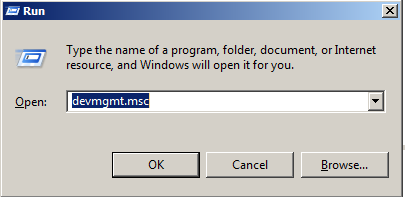
\includegraphics[width=200pt]{images/software/devicemgr}
				\caption{Memanggil Device Manager}
			\end{figure}
			
			\item Tekan (\keys{\return}) atau klik OK
			
			\item Cari entry \textit{Ports (COM and LPT)}.
			Catat nomor port untuk entry \textit{STMicroelectronics Virtual COM Port}.
			Dalam contoh ini, terkonfigurasi pada COM3.
			
			\begin{figure}[H]
				\centering
				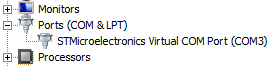
\includegraphics[width=200pt]{images/software/comport}
				\caption{Serial Komunikasi pada COM3}
			\end{figure}
		\end{itemize}
		
		
		\item Install Serial Terminal.
		Untuk dapat berkomunikasi via serial port, perlu diinstall serial terminal.
		Disini dicontohkan menggunakan \textit{Hercules}.
		
		\begin{itemize}
			\item Program terminal Hercules. Dapat didownload di \href{https://drive.google.com/drive/folders/1fgNPnGeSm20TrFfwmeCa4B24WIN_t_o_?usp=share_link}{Terminal}.
			\begin{figure}[H]
				\centering
				
\includegraphics[width=200pt]{images/software/hercules}
				\caption{Hercules Terminal}
			\end{figure}
			
			\item Jalankan program Hercules.
			Jika muncul konfirmasi lisensi, cukup \textit{Close} saja.
			
			\item Pilih tab \textit{Serial}.
			\begin{figure}[H]
				\centering
				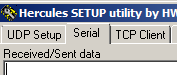
\includegraphics[width=200pt]{images/software/hercules_serial}
				\caption{Serial Terminal}
			\end{figure}
		\end{itemize}
		
		\item Test Komunikasi Serial
		\begin{itemize}
			\item Hercules Serial Terminal
			\begin{figure}[H]
				\centering
				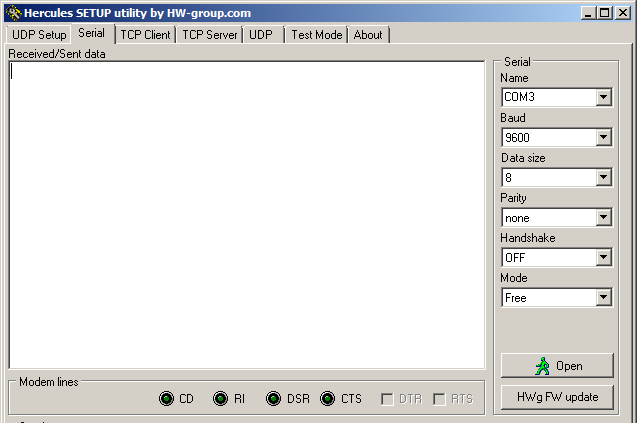
\includegraphics[width=250pt]{images/software/hercules_terminal}
				\caption{Hercules Serial Terminal}
			\end{figure}
			
			\item Setting Port pada Serial Terminal sebagai berikut
			\begin{itemize}
				\item Name     : COM3
				\item Baud     : 9600
				\item Data size: 8
				\item Parity   : none
			\end{itemize}
			
			\begin{figure}[H]
				\centering
				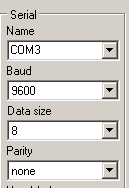
\includegraphics[width=100pt]{images/software/hercules_port}
				\caption{Pengaturan serial port}
			\end{figure}
			
			\item Klik Open (pastikan unit prototype sudah standby dan terhubung
			serta nama COM port sudah sesuai)
			
			\begin{figure}[H]
				\centering
				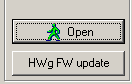
\includegraphics[width=100pt]{images/software/hercules_open}
				\caption{Open Serial Port}
			\end{figure}
			
			\item Kolom terminal akan menampilkan pesan:
			\begin{minted}[frame=lines,framesep=2mm,fontsize=\small]{text}
Serial port COM3 opened
			\end{minted}
			
			\item Selanjutnya, pada kolom terminal,
			masukkan perintah berikut dan diakhiri dengan (\keys{\return})
			\begin{minted}[frame=lines,framesep=2mm,fontsize=\small]{text}
info
			\end{minted}
			Serial akan menampilkan informasi kernel dan platform
			\begin{figure}[H]
				\centering
				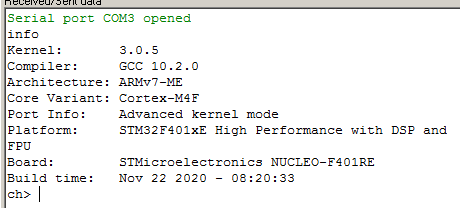
\includegraphics[width=300pt]{images/software/hercules_text}
				\caption{Informasi Platform}
			\end{figure}
		\end{itemize}
		
	\end{enumerate}
	
	Berikut beberapa contoh perintah serial yang dapat diakses melalui komunikasi serial Konsol:
	
	\begin{table}[H]
		\renewcommand{\tablename}{Tabel}
		\centering
		\caption{Contoh perintah serial yang tersedia pada konsol Audiometri. \label{table:serial-code}}
		\begin{tabular}{| p{0.05\textwidth} | p{0.1\textwidth} | p{0.15\textwidth} | p{0.2\textwidth} | p{0.4\textwidth} |}
			\hline
			\textbf{No} & \textbf{Perintah} & \textbf{Fungsi} & \textbf{Contoh Perintah} & \textbf{Contoh Respon} \\
			\hline
			1 & \textit{help} & Menampilkan Perintah yang tersedia & \textit{help} & \textit{coba mmc out tes led sig tone virt ...} \\
			\hline
			2 & \textit{info} & Menampilkan Info Platform Chip & \textit{info} & \textit{Kernel: 6.1.4Compiler: GCC 12.1.0 ...} \\
			\hline
			3 & \textit{mmc} & Mengelola isi SDCard & \textit{mmc} & \textit{usage: mmc [test|ls|lsnum| ...} \\
			& & & \textit{mmc ls} & \textit{HT1.TXT HT2.TXT ...} \\
			& & & \textit{mmc cat 1} & \textit{\{"audiogram":\{ ...} \\
			\hline
			4 & \textit{out} & Menghasilkan nada murni &  \textit{out} & \textit{usage: out <0/1> <freq> <ampl> ...} \\
			& & & \textit{out 500 11} & \textit{Out: Freq:  500 Ampl:11} \\
			& & & \textit{out 1 250 8} & \textit{Out: Freq:  250 Ampl:8} \\
			\hline
		\end{tabular}
	\end{table}
	
	\textbf{Keterangan}: Beberapa keterangan perintah \textit{out}:
	\begin{itemize}
		\item Pilihan Channel adalah 0 atau kosong untuk kiri, dan 1 untuk kanan.
		\item Pilihan Frekuensi Nada Murni: 125Hz, 250Hz, 500Hz, 1000Hz, 2000Hz, 4000Hz, dan 8000Hz.
		\item Pilihan Skala Loudness Nada Murni: 1, 2, 3, 4, 5, 6, 7, 8, 9, 10, dan 11.
	\end{itemize}
	
	\subsubsection{Kalibrasi Hearing Level Air Conduction}
	\label{subsubsec:hl}
	\begin{enumerate}
		\item Pengujian yang dimaksudkan untuk mendapatkan nilai aktual output audio nada murni dalam satuan dBA.
		
		\item Output nada murni memiliki karakteristik:
		\begin{itemize}
			\item frekuensi adalah nilai frekuensi (dalam Hz) yaitu 125, 250, 500, 1000, 2000, 4000, dan 8000.
			\item amplitudo adalah skala amplitudo antara 1 sampai 11.
		\end{itemize}
		
		\item Berikut contoh perintah untuk menghasilkan nada murni (sebagaimana Tabel \ref{table:serial-code}):
		
		\begin{itemize}
			\item Nada murni pada frekuensi 500Hz dan skala 11.
			\begin{minted}[frame=lines,framesep=2mm,fontsize=\small]{text}
out 500 11
			\end{minted}
			
			\item Nada murni pada frekuensi 500Hz dan skala 1.
			\begin{minted}[frame=lines,framesep=2mm,fontsize=\small]{text}
out 500 1
			\end{minted}
			
			\item Nada murni pada frekuensi 500Hz dan skala 11 di channel/sisi kanan.
			\begin{minted}[frame=lines,framesep=2mm,fontsize=\small]{text}
out 1 500 11
			\end{minted}
			
			\textbf{Catatan:} Pengukuran dua sisi diperlukan jika diasumsikan headphone berbeda karakteristik kedua sisinya.
		\end{itemize}
		
		\item Buka terminal serial dan software REW. Pada software REW dan prosedur kalibrasi dilakukan.
		
		\item Pada software REW, buka menu {\bf RTA}. Atur pengaturan dengan menekan simbol {\bf Setting} pada bagian kanan atas menu.
		
		\item Siapkan perangkat audiometer portable. Pada terminal serial, pilih menu {\bf Open}. Tuliskan code untuk membangkitkan nada murni seperti pada langkah 3. Tekan {\bf Enter}.
		
		\item Perhatikan perubahan nilai pada panel {\bf RTA} di software REW. Setelah 5 detik (sesuai dengan durasi nada murni yang dibangkitkan), simpan data peak dengan menekan tombol pada bagian atas panel {\bf RTA}, seperti pada Gambar.
		
		\item Data yang disimpan akan muncul pada panel utama software REW
		
		\item Lakukan prosedur 6-8 secara berurutan pada nilai skala 1 - 11 secara berurutan dan bolak balik sebanyak 3 kali. Prosedur ini juga dapat digunakan untuk memeriksa histeresis dari luaran nada murni audiometer portable. 
		
		\item Prosedur 6-9 dilaksanakan masing-masing untuk pengujjian pada sisi kiri dan kanan dari headphone.
		
		\item Setelah semua pengukuran dilakukan, tutup menu {\bf RTA} dan kembali ke halaman utama. Pada halaman tersebut sudah terdapat beberapa data yang telah disimpan sebelumnya (Gambar).
		
		\item Export seluruh data dalam format .txt dengan memilih menu {\bf File} $\rightarrow$ {\bf Export}  $\rightarrow$ {\bf Export all measurement data in .txt}
		
		\item Untuk memperoleh nilai dBA pada setiap skala dan frekuensi uji, buka file .txt yang disimpan untuk nilai skala dan frekuensi yang hendak diketahui. Catat nilai dBA pada kondisi tersebut pada Tabel \ref{table:data}.
		
		\item Secara menyeluruh, uji nada murni akan mengisi tabel dBA antara frekuensi dan skala seperti Tabel \ref{table:data} berikut:
		
		\begin{table}[H]
			\renewcommand{\tablename}{Tabel}
			\caption{Format tabel hasil uji nada murni \label{table:data}}
			\centering 
			\begin{tabular}{|p{0.07\linewidth}|c|c|c|c|c|c|c|c|c|c|c|}
				\hline
				Scale/ Freq & 11 & 10 & 9 & 8 & 7 & 6 & 5 & 4 & 3 & 2 & 1\\ [0.5ex]
				\hline\hline
				125Hz & x dBA & x dBA & x dBA & x dBA & x dBA & x dBA & x dBA & x dBA & x dBA & x dBA & x dBA\\
				\hline
				250Hz & x dBA & x dBA & x dBA & x dBA & x dBA & x dBA & x dBA & x dBA & x dBA & x dBA & x dBA\\
				\hline
				500Hz & x dBA & x dBA & x dBA & x dBA & x dBA & x dBA & x dBA & x dBA & x dBA & x dBA & x dBA\\
				\hline
				1000Hz & x dBA & x dBA & x dBA & x dBA & x dBA & x dBA & x dBA & x dBA & x dBA & x dBA & x dBA\\
				\hline
				2000Hz & x dBA & x dBA & x dBA & x dBA & x dBA & x dBA & x dBA & x dBA & x dBA & x dBA & x dBA\\
				\hline
				4000Hz & x dBA & x dBA & x dBA & x dBA & x dBA & x dBA & x dBA & x dBA & x dBA & x dBA & x dBA\\
				\hline
				8000Hz & x dBA & x dBA & x dBA & x dBA & x dBA & x dBA & x dBA & x dBA & x dBA & x dBA & x dBA\\
				\hline
			\end{tabular}
		\end{table}
	\end{enumerate}
	
	
	
	\subsubsection{Kalibrasi Akurasi Frekuensi}
	\begin{enumerate}
		\item Pengujian dimaksudkan untuk mendapatkan nilai selisih antara frekuensi target dengan frekuensi yang terukur. 
		\item Prosedur mengikuti langkah 6-8 pada pengujian kalibrasi hearing level air conduction (bagian \ref{subsubsec:hl})
		\item Nilai selisih frekuensi diperoleh dengan model matematis berikut
		\begin{equation}
			\label{eq:af}
			C = f_{std} - f_{audiometer}
		\end{equation}
		dimana, 
		
		\begin{tabular}{p{.15\textwidth} p{.01\textwidth} p{.5\textwidth}}
			\(C\) & : & Koreksi penunjukan frekuensi pada audiometer \\
			\(f_{std}\) & : & Nilai frekuensi yang terukur pada standar (terukur) \\
			\(f_{audiometer}\) & : & Nilai frekuensi yang ditampilkan oleh audiometer (target) \\
		\end{tabular}
	
		\item Persamaan \ref{eq:af} diterapkan pada perhitungan di setiap level dan di setiap frekuensi, masing-masing untuk pengujian pada sisi kiri dan kanan headphone.
		
		\item Hasil perhitungan kemudian dimasukkan ke dalam Tabel \ref{table:af-data} pengujian berikut.
		
		\begin{table}[H]
			\renewcommand{\tablename}{Tabel}
			\caption{Format tabel hasil uji akurasi frekuensi \label{table:af-data}}
			\centering
			\begin{tabular}{|p{0.07\linewidth}|c|c|c|c|c|c|c|c|c|c|c|}
				\hline
				Scale/ Freq & 11 & 10 & 9 & 8 & 7 & 6 & 5 & 4 & 3 & 2 & 1\\ [0.5ex]
				\hline\hline
				125Hz & x Hz & x Hz & x Hz & x Hz & x Hz & x Hz & x Hz & x Hz & x Hz & x Hz & x Hz\\
				\hline
				250Hz & x Hz & x Hz & x Hz & x Hz & x Hz & x Hz & x Hz & x Hz & x Hz & x Hz & x Hz\\
				\hline
				500Hz & x Hz & x Hz & x Hz & x Hz & x Hz & x Hz & x Hz & x Hz & x Hz & x Hz & x Hz\\
				\hline
				1000Hz & x Hz & x Hz & x Hz & x Hz & x Hz & x Hz & x Hz & x Hz & x Hz & x Hz & x Hz\\
				\hline
				2000Hz & x Hz & x Hz & x Hz & x Hz & x Hz & x Hz & x Hz & x Hz & x Hz & x Hz & x Hz\\
				\hline
				4000Hz & x Hz & x Hz & x Hz & x Hz & x Hz & x Hz & x Hz & x Hz & x Hz & x Hz & x Hz\\
				\hline
				8000Hz & x Hz & x Hz & x Hz & x Hz & x Hz & x Hz & x Hz & x Hz & x Hz & x Hz & x Hz\\
				\hline
			\end{tabular}
		\end{table}
		
	\end{enumerate}
	
	\subsubsection{Kalibrasi Total Harmonic Distortion Air Conduction}
	\begin{enumerate}
		\item Pengujian dimaksudkan untuk mendapatkan nilai selisih antara frekuensi target dengan frekuensi yang terukur. 
		\item Prosedur mengikuti langkah 6-8 pada pengujian kalibrasi hearing level air conduction (bagian \ref{subsubsec:hl}) 		
		\item Nilai selisih frekuensi diperoleh dengan model matematis berikut
		\begin{equation}
			\label{eq:thd}
			C = THD_{std} - THD_{audiometer}
		\end{equation}
		dimana, 
		
		\begin{tabular}{p{.15\textwidth} p{.01\textwidth} p{.7\textwidth}}
			\(C\) & : & Koreksi penunjukan total harmonic distortion pada audiometer \\
			\(THD_{std}\) & : & Nilai total harmonic distortion yang terukur pada standar (terukur) \\
			\(THD_{audiometer}\) & : & Nilai total harmonic distortion yang ditampilkan oleh audiometer (target) \\
		\end{tabular}
		
		\item Persamaan \ref{eq:thd} diterapkan pada perhitungan di setiap level dan di setiap frekuensi, masing-masing untuk pengujian pada sisi kiri dan kanan headphone.
		
		\item Hasil perhitungan kemudian dimasukkan ke dalam Tabel \ref{table:thd-data} pengujian berikut.
		
		\begin{table}[H]
			\renewcommand{\tablename}{Tabel}
			\caption{Format tabel hasil uji akurasi frekuensi \label{table:thd-data}}
			\centering
			\begin{tabular}{|p{0.07\linewidth}|c|c|c|c|c|c|c|c|c|c|c|}
				\hline
				Scale/ Freq & 11 & 10 & 9 & 8 & 7 & 6 & 5 & 4 & 3 & 2 & 1\\ [0.5ex]
				\hline\hline
				125Hz & x \% & x \% & x \% & x \% & x \% & x \% & x \% & x \% & x \% & x \% & x \%\\
				\hline
				250Hz & x \% & x \% & x \% & x \% & x \% & x \% & x \% & x \% & x \% & x \% & x \%\\
				\hline
				500Hz & x \% & x \% & x \% & x \% & x \% & x \% & x \% & x \% & x \% & x \% & x \%\\
				\hline
				1000Hz & x \% & x \% & x \% & x \% & x \% & x \% & x \% & x \% & x \% & x \% & x \%\\
				\hline
				2000Hz & x \% & x \% & x \% & x \% & x \% & x \% & x \% & x \% & x \% & x \% & x \%\\
				\hline
				4000Hz & x \% & x \% & x \% & x \% & x \% & x \% & x \% & x \% & x \% & x \% & x \%\\
				\hline
				8000Hz & x \% & x \% & x \% & x \% & x \% & x \% & x \% & x \% & x \% & x \% & x \%\\
				\hline
			\end{tabular}
		\end{table}
		
	\end{enumerate}

	\newpage
	\section{Hasil Pengujian}

	\subsection{Pemeriksaan Fisik dan Fungsi}
	
	
	\subsection{Pengujian Keselamatan Listrik}
	
	
	\subsection{Pengujian Kinerja}
	\subsubsection{Hearing Level Air Conduction}
	
	\subsubsection{Akurasi Frekuensi}
	
	\subsubsection{Total Harmonic Distortion}


\end{document}
